\documentclass[12pt]{article}
\usepackage[left=20mm, top=20mm, right=20mm, bottom=20mm, headsep=10pt]{geometry} 
\usepackage{cmap} % для кодировки шрифтов в pdf
\usepackage[T2A]{fontenc}
\usepackage[utf8]{inputenc}
\usepackage[russian]{babel}
\usepackage{graphicx} % для вставки картинок
\usepackage{amssymb,amsfonts,amsmath,amsthm,amsbsy} % математические дополнения от АМС
\usepackage{mathtools}
\usepackage{indentfirst} % отделять первую строку раздела абзацным отступом тоже
\usepackage{multicol}
%\usepackage{tempora}
\usepackage{epstopdf}
\usepackage{svg}
\usepackage{mathtools}
\usepackage{framed}
\usepackage{wrapfig}
\usepackage[font=small]{caption}
\usepackage{floatrow}
\floatsetup[table]{capposition=top}
\usepackage{subcaption}
\usepackage{titlesec}
\usepackage{setspace}
\usepackage{enumitem}
\usepackage{float}
\usepackage{epstopdf}
\usepackage{hepunits}
\usepackage[final]{pdfpages}
\usepackage{tikz}
\usepackage{authblk}
\usepackage{physics}
\usepackage{upgreek}
\usepackage{cancel} 

\newcommand{\longeq}{\scalebox{3}[1]{=}}

\usetikzlibrary{positioning,shapes,arrows,decorations.pathmorphing}
%opening

\makeatletter
\renewcommand\AB@affilsepx{, \protect\Affilfont}
\makeatother

\title{Обратное комптоновское рассеяние. История эффекта. Угловые распределения в собственной и лабораторной системах отсчета}
\author{Степан Захаров}
\begin{document}
\maketitle

\vspace{-3em} 
%\begin{abstract}
%\end{abstract}

\section{История эффекта}
Взаимодействие электромагнитного излучения с веществом интересовало ученых ещё с середины  XIX века, когда Максвеллом была создана довольно стройная теория электромагнитизма. Череда открытий в физике частиц на рубеже XIX-XX  вв. окончательно сформировала понимание об электромагнитном излучении, как о потоке безмассовых частиц с нулевым электрическим зарядом и отличных от нуля энергией и импульсом --- фотонах. Взаимодействие же фотонов с электронами вещества (которые были открыты примерно в это же время) было описано в работах Дж. Дж. Томсона, который предположил, что заряд, взаимодействия с электромагнитной волной, испытывает ускорение и излучает вторичную волну во всех направлениях. Сечение рассеяния описывается формулой:
\begin{equation}
	\frac{d \sigma_{_T}}{d\Omega} = \frac{e^4}{m_e^2 c^4} \big(1-\cos^2\theta\big) = \bigg\{r_e = \frac{e^2}{m_e c^2} \bigg\} = r_e^2\big(1+\cos^2\theta\big).
	\label{eq:tomson_xsec}
\end{equation}
Видно, что сечение не зависит от энергии падающего фотона. Данное объяснение имело хорошее согласие с экспериментом в области энергий фотонов $\hbar \omega_0 \ll m_e c^2$. Однако при увеличении энергии падающего фотона, предсказания классической томсоновской теории начинали расходиться с экспериментом. В добавок, энергия рассеянного фотона изменялась, чего не предсказывала теория Томсона. Дальнейшее исследование, которое провел А. Комптон показало, что эффект изменения частоты рассеянных фотонов зависит как от энергии падающих фотонов, так и от угла рассеяния. 
Сечение комптоновского рассеяния имеет похожую угловую зависимость с томсоновским сечением:
\begin{equation}
\frac{d \sigma_{_K}}{d\Omega} = \frac{r_e^2}{2} \bigg[\frac{\omega'}{\omega}\bigg]^2 \bigg(\frac{\omega'}{\omega}+\frac{\omega}{\omega'} - \sin^2\theta\bigg). 
\label{eq:compton_xsec}
\end{equation}
В формуле \ref{eq:compton_xsec}: $\omega'$ -- частота рассеянного фотона, которая определяется из законов сохранения импульса и энергии, через частоту падающего $\Omega$ фотона и угол рассеяния между падающим и рассеянным фотоном $\theta$:
\begin{equation}
\omega' = \frac{\omega }{1+\frac{\omega}{m_e c^2}(1-\cos \theta)}.
\label{eq:gam2_freq}
\end{equation}
Отметим, что параметр малости $\hbar \omega_0 / m_e c^2 \ll 1$ напрямую входит в формулу \ref{eq:gam2_freq} и определяет переход от комптоновского сечения к томсоновскому. \par
Отдельно стоит рассмотреть случай, когда происходит процесс рассеяния оптических фотонов на ультрарелятивистских электронах. Характерные значения энергий в лабораторной системе отсчета : 
\begin{itemize}
	\item Энергия падающего фотона $\omega_0 \sim 2~\eV$
	\item Энергия электрона $E_e \sim 5~\GeV$ ($\gamma \sim 10^4$)
\end{itemize}
\par В контексте работы нас интересует вид угловых распределений рассеянных фотонов. Для этого необходимо получить выражение для дифференциального сечения \ref{eq:compton_xsec} в лабораторной системе отсчета. Удобно сначала получить вид сечения в системе покоя электрона, а затем перейти в лабораторную систему отсчета. Введем систему координат для задачи: ось $z$ направим против направления движения фотона, оси $x$ и $y$ сориентируем так, чтобы тройка векторов $xyz$ была правой, а также чтобы рассеяние происходило в плоскости $xOz$:
\begin{figure}[H]
	\begin{tikzpicture}[
	>=stealth',
	pos=.8,
	photon/.style={decorate,decoration={snake,post length=1mm}}]
	\draw[->, -latex] (-5,0) -- (-4,0) node[sloped, below] {\footnotesize{z}};
	\draw[->, -latex] (-5,0) -- (-5,1) node[sloped, right] {\footnotesize{x}};
	\draw[->, -latex] (-5,0) -- (-5-0.5,-0.5) node[right=0.3ex] {\footnotesize{$y$}};
'
	\draw[->, latex-] (-2,-0.7) -- (-0.25,-.05) node[sloped, below, midway] {$e^{-}{'} (E',\textbf{p}')$};
	\draw[->,photon] (4,0) -- (0.25,0) node[sloped, below, midway] {$\gamma (\omega, \textbf{k})$};
	\draw[->,photon] (0.25,0.12) -- (4,1.5) node[sloped,above, midway] {$\gamma' (\omega', \textbf{k}')$};
	\filldraw[black] (0,0) circle (2pt) node[anchor=south east] {$e^- (m,\textbf{0})$};
	\draw (3.1,0) arc (0:21:3) node[anchor=west , midway] {$\chi = \pi - \theta$};
	\end{tikzpicture}\\
	\caption{Кинематика комптоновского рассеяния в системе покоя электрона.}
\end{figure}
Зафиксируем обозначения: частицы в начальном состоянии --- без штриха, в конечном --- со штрихом. Обычно за угол рассеяния принимают угол между начальным и конечным фотонами $\theta$, но, учитывая тот факт, что начальный электрон ультрарелятивистский, можно ожидать сильный буст сечения в правое полупространство. Поэтому удобно работать с углом отлета фотона $\chi$. 
\par Поляризации частиц будем обозначать следующим образом: поляризация фотона описывается вектором Стокса $\vec{\xi} = [\xi_0,\xi_1,\xi_2,\xi_3]=[I,Q,U,V]$. Его компоненты задаются соотношением амплитуд и сдвиг фаз по главным осям системы. Если амплитуды электромагнитного поля имеют проекции на главные оси: $E_x$ и $E_y$, а разность фаз между ними -- $\psi$, то выражения для стоксовских параметров следующие: 
\begin{equation}
	\begin{split}
	I &= E_x^2 + E_y^2\\
	Q &= E_x^2 - E_y^2\\
	U &= 2E_x E_y \cos \psi\\
	V &= 2E_x E_y \sin \psi.
	\end{split}
	\label{eq:stokes_pars}
\end{equation}
Удобно также нормировать вектор Стокса на значение полной интенсивности $I = E_x^2 + E_y^2$. Тогда остальные параметры будут изменяться в пределах $[-1,+1]$. 
Поляризацию же электронного пучка принято определять как направление спина, усредненное по всем электронам в пучке: $\vec{\zeta} = [\zeta_1,\zeta_2,\zeta_3]$; компоненты вектора есть проекции среднего спина на главные оси системы.  


\subsection{Случай неполяризованных электронов}
Если начальный пучок электронов не поляризован, то сечение рассеяния будет зависеть только от поляризации оптических фотонов $\vec{\xi}$. Для начала необходимо учитывать степень поляризации фотонов. Пусть фотоны поляризованы линейно по одной из главных осей. Тогда степень поляризации будет дополнительным множителем последнего члена в формуле \ref{eq:compton_xsec} :

\begin{equation}
\frac{d \sigma_{_K}(\vec{\xi})}{d\Omega} = \frac{r_e^2}{2} \bigg[\frac{\omega'}{\omega}\bigg]^2 \bigg(\frac{\omega'}{\omega}+\frac{\omega}{\omega'} -(1-\xi_1) \sin^2\theta\bigg). 
\label{eq:compton_xsec_pol1}
\end{equation}
В общем случае поляризация фотонов может иметь произвольное направление. Параметры $\xi_1$ и $\xi_2$ однозначно, но неявно задают полную степень поляризации и угол поворота плоскости поляризации к главным осям. Cечение же зависит только от полной степени линейной поляризации $\xi_{lin}$. В связи с этим удобно выделить явно полную степень и угол поворота плоскости поляризации, основываясь на выводе, проведенном в главе [ВСТАВИТЬ ССЫЛКУ НА ФОРМУЛУ 6 ИЗ ГЛАВЫ ПРО КОРРЕКЦИЮ ОПТИКИ]:
\begin{align}
\xi_{lin} &= \sqrt{\xi_1^2+\xi_2^2}\\
\varphi_0 &= \pi/4 - \frac{1}{2}\atan\bigg(\frac{Q}{U}\bigg).
\end{align}
Наличие поворота плоскости поляризации к главным осям вызывает появление дополнительной угловой зависимости от азимутального угла $\varphi$:
\begin{equation}
\frac{d \sigma_{_K}(\vec{\xi})}{d\Omega} = \frac{r_e^2}{2} \bigg[\frac{\omega'}{\omega}\bigg]^2 \bigg(\frac{\omega'}{\omega}+\frac{\omega}{\omega'} -\big(1-\xi_{lin}\cos(2[\varphi - \varphi_0])\big) \sin^2\theta\bigg). 
\label{eq:compton_xsec_pol2}
\end{equation}
\par Данное выражение представляет собой дифференциальное сечение комптоновского рассеяния поляризованного фотона на неполяризованном электроне в системе покоя электрона. Чтобы получить его вид в лабораторной системе отсчета, необходимо выполнить преобразования Лоренца для всех входящих в него величин. Перед этим условимся величины, выраженные в лабораторной системе отсчета обозначать индексом $x_\text{л}$, а в системе покоя электрона --- без индекса. Относительное движение системы покоя электрона и лабораторной системы описывается $\gamma$--фактором:
\begin{equation}
\gamma = \frac{1}{\sqrt{1-\beta}} = \frac{E_{e}}{m_{e}}, \qquad \beta = \frac{v_{{e}}}{c}
\label{eq:gam_beta_def}
\end{equation}
В дальнейших расчетах пользуемся системой единиц Хевисайда, где $\hbar=c=e=1$. Найдем выражения для четырехимпульсов начальных частиц:
\begin{equation}
k_{\text{л}} = \omega\big(1,0,0,-1\big), \qquad p_{\text{л}} = E_e\big(1,0,0,\beta\big)
\label{eq:initial_state_particles}
\end{equation}
В системе покоя электрона четырехимпульс фотона имеет вид:
\begin{equation}
k= \gamma(1+\beta) \omega\big(1,0,0,-1\big)
\end{equation}
Рассеянный фотон имеет импульс под углом к оси $z$, значит необходимо отдельно преобразовать параллельную и перпендикулярную компоненты:
\begin{align}
\omega' &= \gamma\big(\omega'_{\text{л}} - \beta k'_{z\text{л}}\big) =  \gamma\omega'_{\text{л}}\big(1 - \beta \cos\chi_{\text{л}}\big)\label{eq:gam2_boost_start}\\
k_z' &= \gamma\big(k_{z\text{л}} - \beta\omega'_{\text{л}} \big) =  \gamma\omega'_{\text{л}}\big(\beta\cos\chi_{\text{л}} - 1\big)\\
k_x' &= k_{x\text{л}}' =  \omega' \sin \chi_{\text{л}}
\label{eq:gam2_boost_end}
\end{align}
Используя предыдущие формулы, найдем выражения для преобразования косинуса и синуса угла отлета фотона:
\begin{align}
\cos \chi &= \frac{k_z'}{\omega'} = \frac{\cos\chi_{\text{л}} - \beta}{1 - \beta \cos \chi_{\text{л}}}, \qquad 1 + \cos \chi = \frac{(1-\beta)(1+ \cos\chi_{\text{л}})}{1 - \beta \cos \chi_{\text{л}}}\label{eq:gam2_angle_start} \\
\sin \chi &= \frac{k_x'}{\omega'} = \frac{\sin\chi_{\text{л}}}{\gamma (1 - \beta \cos \chi_{\text{л}})}
\label{eq:gam2_angle_end}
\end{align}
Используем формулу \ref{eq:gam2_freq} и преобразуем сечение \ref{eq:compton_xsec_pol2} так, чтобы оно было выражено через частоту начального фотона и угол отлета конечного фотона уже в лабораторной системе отсчёта. Для этого можно сначала поработать с параметром $\omega/\omega'$:
\begin{equation}
\begin{split}
\frac{\omega}{\omega'} &= 1 + \frac{\omega}{m_e}(1+cos\chi) = 1 + \frac{[\gamma(1+\beta)\omega]}{m_e}\frac{(1-\beta)(1+ \cos\chi_{\text{л}})}{1 - \beta \cos \chi_{\text{л}}}  
\\ &= 1 + \frac{\omega}{\gamma m_e}\frac{(1+ \cos\chi_{\text{л}})}{1 - \beta \cos \chi_{\text{л}}} \simeq 1 + \frac{\omega}{\gamma m_e}\frac{(1+ 1 - \chi_{\text{л}}^2/2)}{1 - \beta (1- \chi_{\text{л}}^2/2)} \stackrel{\cdot 2/2}{\longeq} 1 + \frac{\omega}{\gamma m_e}\frac{(4 - \chi_{\text{л}}^2)}{\underbrace{2(1 - \beta)}_{=1/\gamma^2}+ \underbrace{\beta \chi_{\text{л}}^2}_{\sim \big(1 - \frac{1}{2\gamma^2}\big)\frac{1}{\gamma^2}}} 
\\&\simeq
\frac{1/\gamma^2 + \chi_{\text{л}}^2 + \frac{4\omega}{\gamma m_e}}{1/\gamma^2 + \chi_{\text{л}}^2} \stackrel{\cdot \gamma^2}{\longeq}  \frac{1 + \gamma^2\chi_{\text{л}}^2 + \frac{4\gamma\omega}{ m_e}}{1 + \gamma^2\chi_{\text{л}}^2} = 
\bigg\{ \begin{matrix}\eta = \gamma\chi_{\text{л}} \\ \kappa = \frac{4\gamma\omega}{ m_e}\end{matrix}\bigg\} = \frac{1+\eta^2+ \kappa}{1+\eta^2}.
\end{split}
\end{equation}
Итак, мы получили выражение для отношения частот начального и конечного фотонов, выраженное через два безразмерных параметра: $\eta$ угол отлета фотона в единицах $\gamma$ и $\kappa$  ---  параметр жесткости начального фотона. Стоит отметить, что расчет проведен для ультрарелятивистского случая, когда $\chi_{\text{л}} \sim 1/\gamma \sim 10^{-4}$, поэтому членами $\sim 1\gamma^4$ можно пренебречь. 
\par По аналогии с преобразованиями выше, выразим оставшиеся параметры в сечении:
\begin{equation}
\begin{split}
\sin^2 \chi &= \frac{\sin^2\chi_{\text{л}}}{\gamma^2 (1 - \beta \cos \chi_{\text{л}})^2} \simeq
\frac{\chi_{\text{л}}^2}{\gamma^2 \big(1 - \beta(1- \chi_{\text{л}}^2/2)\big)^2} \simeq	 \frac{4\chi_{\text{л}}^2}{\gamma^2 (1/\gamma^2 +\chi_{\text{л}}^2)^2} = 
\frac{4\eta^2}{(1+\eta^2)^2} 
\end{split}
\end{equation}

\begin{equation}
d\Omega = \sin \chi d\chi d\varphi \simeq \frac{4\eta d\eta d\varphi}{(1+\eta^2)^2} = \frac{4\gamma^2}{ (1+\eta^2)^2} \underbrace{\sin \chi_{\text{л}} d\chi_{\text{л}} d\varphi}_{d \Omega_{\text{л}}}
\end{equation}
Теперь можно выписать вид сечения комптоновского рассеяния на неполяризованных электронах в лабораторной системе отсчёта:
\begin{equation}
\begin{split}
\frac{d \sigma_{_K}(\vec{\xi})}{d\Omega_{\text{л}}} = 2\gamma^2 r_e^2 \bigg[\frac{1}{1+\eta^2+\kappa}\bigg]^2 \bigg( 2 + \frac{\kappa^2}{(1+\eta^2)(1+\eta^2+\kappa)} - \frac{4\eta^2}{(1+\eta^2)^2} \big(1-\xi_{lin}\cos(2[\varphi - \beta])\big)\bigg) \\
\end{split}
\label{eq:compton_xsec_noEpol_lrf}
\end{equation}
\subsection{Полностью поляризованный случай}
В современных ускорителях пучки электронов довольно быстро поляризуются из-за синхротронного излучения при движении по криволинейной орбите. Сечение рассеяния в таком случае будет зависеть как от поляризации электронов, так и от поляризации фотонов. Вклад, связанный с поляризацией электронов можно представить как добавку к сечению рассеяния поляризованных фотонов на неполяризованных электронах: 

\begin{equation}
\begin{split}
\frac{d \sigma_{_K}(\vec{\xi},\vec{\zeta})}{d\Omega} = \frac{d \sigma_{_K}(\vec{\xi})}{d\Omega} + \frac{r_e^2}{2} \bigg[\frac{\omega'}{\omega}\bigg]^2 \xi_3 \vec{f} \cdot \vec{\zeta}, \qquad \vec{f} = -\frac{1+\cos \chi_{\text{л}}}{m_e}(\mathbf{k}' - \mathbf{k}\cos \chi_{\text{л}})
\end{split}
\label{eq:comp_xsec_epol_erf}
\end{equation}
В нашем случае пучок электронов поляризуется против направления магнитного поля, поэтому вектор $\vec{\xi} = [-P,0,0]$, где $P$ - степень поляризации. Учитывая, что импульс начального фотона направлен по оси $z$, можем по ортогональности исключить из $\vec{f}$ член, пропорциональный $\mathbf{k}$. Далее переходим в лабораторную систему аналогично случаю, рассмотренному выше:

\begin{equation}
\begin{split}
\vec{f} \cdot \vec{\zeta} &= -\frac{1+\cos \chi_{\text{л}}}{m_e}\mathbf{k}'\cdot\vec{\zeta} = \frac{P}{m_e}\cdot  \underbrace{(1+\cos \chi_{\text{л}})}_{\frac{2}{1+\eta^2}}\cdot  \underbrace{\sin \chi}_{\frac{2\eta}{1+\eta^2}} \cdot\underbrace{\frac{ \omega }{1+\frac{\omega}{m}\big(1+\cos \chi\big)}}_{ 2\gamma\omega_{\text{л}}\frac{1+\eta^2}{1+\eta^2+ \kappa}} = \\
&= \frac{8\omega_{\text{л}}P}{m_e} \frac{\eta}{(1+\eta^2)(1+\eta^2+ \kappa)}
\end{split}
\end{equation}
Подставим полученный ответ в \ref{eq:comp_xsec_epol_erf}, не забудем преобразовать элемент телесного угла и получим вид сечения в случае поляризованных электронов.
\begin{equation}
\begin{split}
\frac{d \sigma_{_K}(\vec{\xi},\vec{\zeta})}{d\Omega_{\text{л}}} &= 
\frac{d \sigma_{_K}(\vec{\xi})}{d\Omega_{\text{л}}} 
+ \frac{r_e^2}{2} \frac{8\gamma\omega_{\text{л}}P \xi_3 }{m_e}
\bigg[\frac{{\cancel{1+\eta^2}}}{1+\eta^2+ \kappa}\bigg]^2\ 
\frac{\eta}{(1+\eta^2)(1+\eta^2+ \kappa)} \frac{4\gamma^2}{\cancel{(1+\eta^2)^2}}= \\
 &=\frac{d \sigma_{_K}(\vec{\xi})}{d\Omega_{\text{л}}} 
 + 4\gamma^2 r_e^2 \kappa P V \frac{\eta}{(1+\eta^2)(1+\eta^2+ \kappa)^3}
\end{split}
\end{equation}
Проанализируем полученное сечение. Неполяризованная его часть представляет собой куполообразную функцию с максимумом в нуле.
\begin{figure}[H]
	\begin{subfigure}{.5\textwidth}
		\centering
		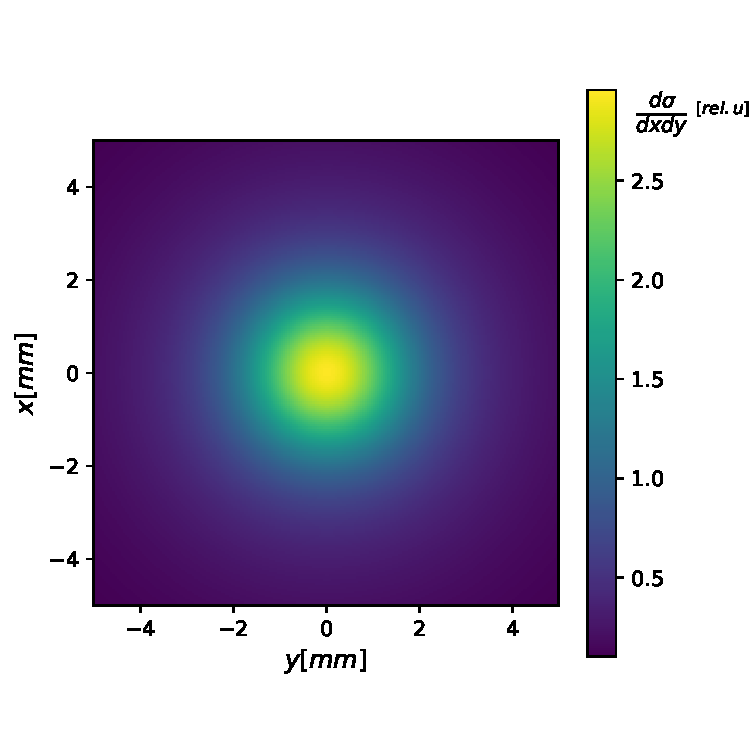
\includegraphics[width=0.8\linewidth]{img/compton_dsdo_nopol}
		\caption{Дифференциальное сечение комптоновского рассеяния в неполяризованном случае}
		\label{fig:dsdxdy_nopol}
	\end{subfigure}%
	\begin{subfigure}{.5\textwidth}
		\centering
		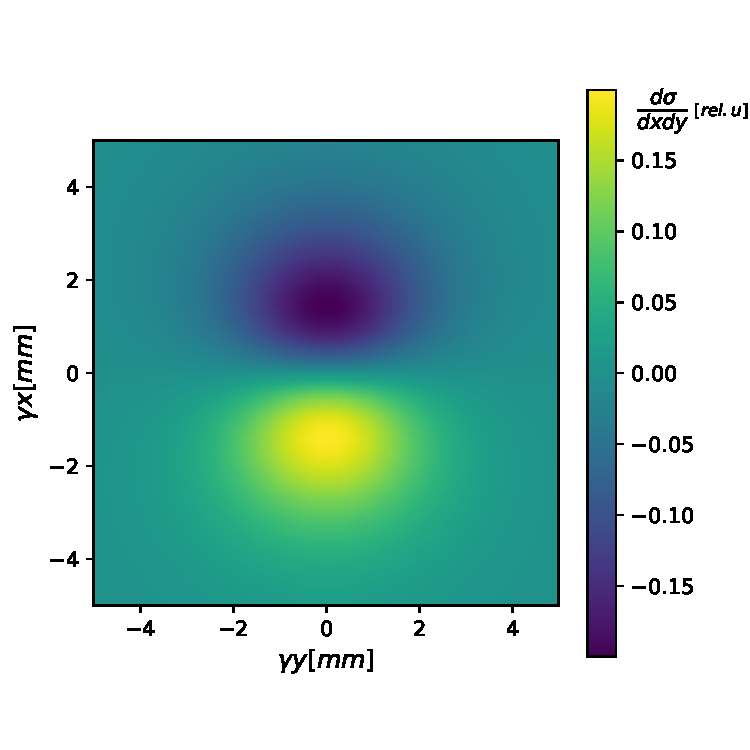
\includegraphics[width=0.8\linewidth]{img/compton_dsdo_diff_v1}
		\caption{Разница сечений комптоновского рассеяния для фотонов с $V=\pm1$}
		\label{fig:dsdxdy_dV1}
	\end{subfigure}
	\caption{Дифференциальные сечения обратного комптоновского рассеяния}
	\label{fig:1}
\end{figure}
Вклад в сечение члена, отвечающего за наличие у электронного пучка поляризации мал по сравнению с остальными членами, однако его можно выделить, если рассматривать разницу сечений для фотонов с левой и правой циркулярными поляризациями. Тогда распределение будет иметь явную асимметрию в направлении среднего спина электронов в пучке (в случае задачи по оси $x$)
\par Наличие у фотонов линейной поляризации вызывает появление квадрупольного члена по азимутальному углу. Это сильно искажает картину и при определенных условиях может как нивелировать эффект от поляризации пучка, так и вызвать появление ложного эффекта.
\begin{figure}[H]
	\begin{subfigure}{.5\textwidth}
		\centering
		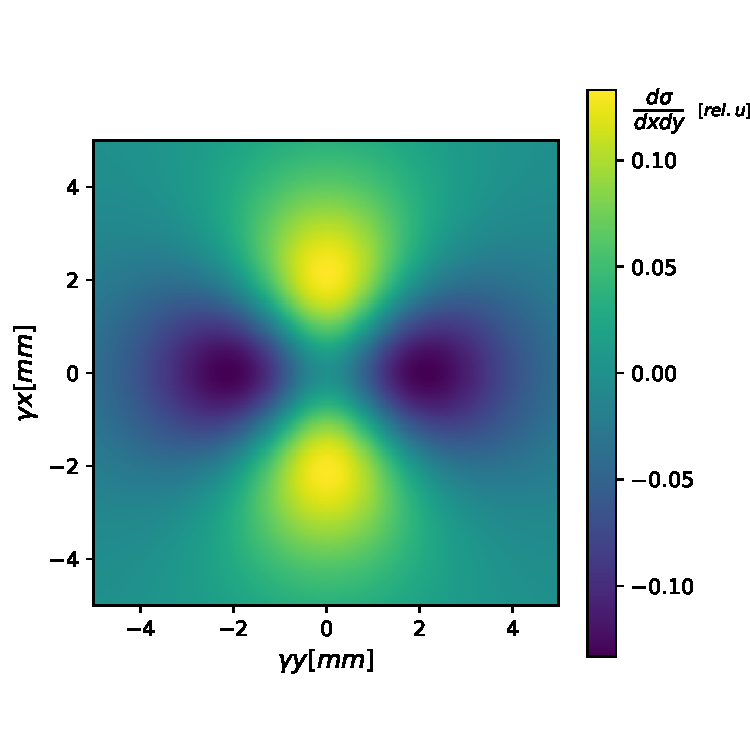
\includegraphics[width=0.8\linewidth]{img/compton_dsdo_diff_q0p1}
		\caption{Разница сечений комптоновского рассеяния для фотонов с $\xi_{lin}=\pm0.1$}
		\label{fig:dsdxdy_dQ0.1}
	\end{subfigure}%
	\begin{subfigure}{.5\textwidth}
		\centering
		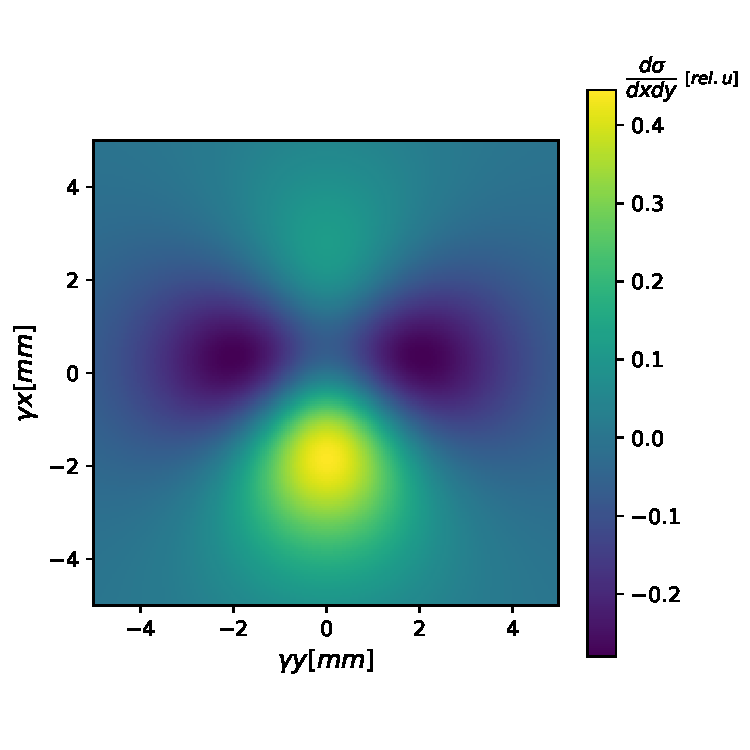
\includegraphics[width=0.8\linewidth]{img/compton_dsdo_diff_q0p1_v1}
		\caption{Разница сечений комптоновского рассеяния для фотонов с $V=\pm1$ и $\xi_{lin}=\pm0.2$ }
		\label{fig:dsdxdy_dQ0.1&dV=1}
	\end{subfigure}
	\caption{Дифференциальные сечения обратного комптоновского рассеяния}
	\label{fig:fig}
\end{figure}




 

















\newpage
\vfill
\end{document}
